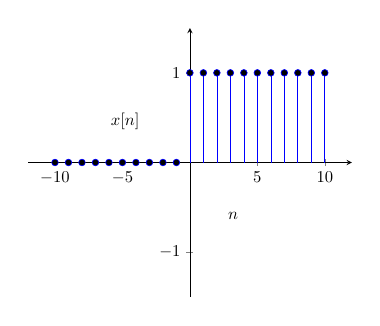
\begin{tikzpicture}[scale=0.6]
\begin{filecontents}{step.dat}
n	xn
-10	0
-9	0
-8	0
-7	0
-6	0
-5	0
-4	0
-3	0
-2	0
-1	0
0	1
1	1
2	1
3	1
4	1
5	1
6	1
7	1
8	1
9	1
10	1
\end{filecontents}
\begin{axis}
[%%%%%%%%%%%%%%%%%%%%%%%%%%%%%%%%%%%
    scale=1,
    axis x line=middle,
    axis y line=middle,
    every axis plot post/.style={mark options={fill=black}},
    xmin=-12,
    xmax=12,
    %xtick={1, 2, 3, 4},
    %xticklabels={1, 2, 3, 4},
    %extra x ticks={-4, -3, -2, -1},
   % extra x tick labels={-4, -3, -2, -1},
   % extra x tick style={ xticklabel style={yshift=0.5ex, anchor=south} },
    xlabel={$n$},
    ylabel={$x[n]$},
    %ytick={-2,-1, 0, 1, 2},
    %xticklabels=\empty,
    ymin=-1.5,
    ymax=1.5,
        x label style={at={(current axis.right of origin)},anchor=west},
        y label style={at={(current axis.above origin)}, anchor=south},
]
\addplot+[ycomb,blue] table [x={n}, y={xn}] {step.dat};
\end{axis}
\end{tikzpicture} 